% *********************************************************************
% © 2026 Jeremy Sylvestre
%
% Permission is granted to copy, distribute and/or modify this document
% under the terms of the GNU Free Documentation License, Version 1.3 or
% any later version published by the Free Software Foundation; with no
% Invariant Sections, no Front-Cover Texts, and no Back-Cover Texts. A
% copy of the license is included in the appendix entitled “GNU Free
% Documentation License” that appears in the output document of this
% PreTeXt source code. All trademarks™ are the registered® marks of
% their respective owners.
%
% *********************************************************************
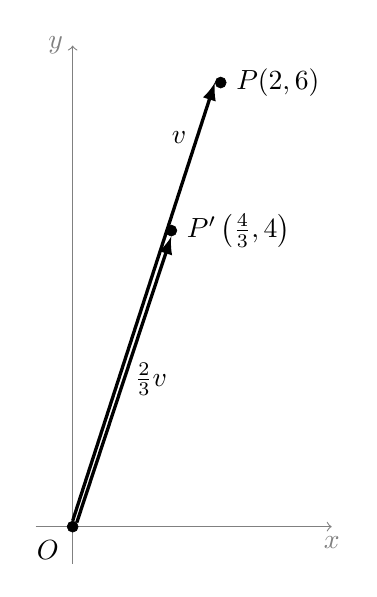
\begin{tikzpicture}[
	point/.style={circle,draw,very thin,fill,inner sep=0pt,minimum size=4pt},
	vector/.style={-latex,very thick},
	scale=0.94
]
	\draw[gray,->] (-0.5,0) to (3.5,0) node[below] {$x$};
	\draw[gray,->] (0,-0.5) to (0,6.5) node[left] {$y$};

	\node[point] at (0,0) (o) [label=below left:$O$] {};
	\node[point] at (2,6) (p) [label=right:{$P(2,6)$}] {};
	\draw[vector] (o.north) to node[left,very near end] {$\uvec{v}$} (p.west);
	\node[point] at (1.333,4) (pp) [label=right:{$P'\left(\frac{4}{3},4\right)$}] {};
	\draw[vector] (o.north east) to node[right] {$\frac{2}{3} \uvec{v}$} (pp.south);

\end{tikzpicture}
